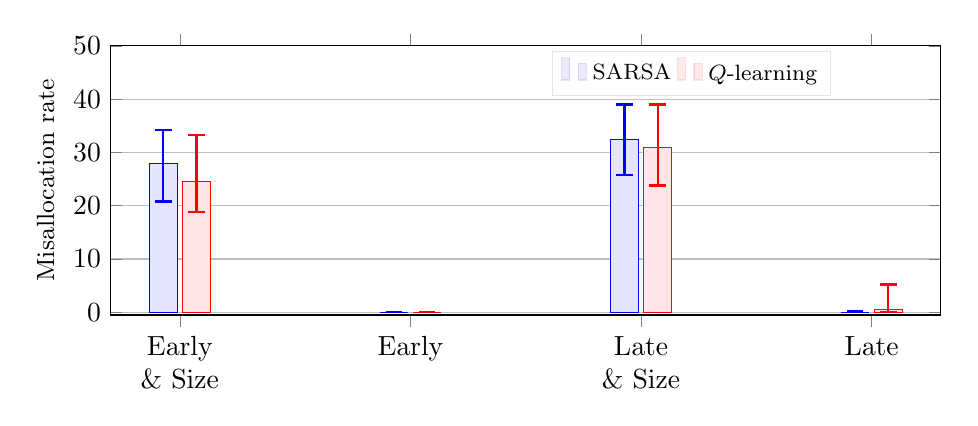
\begin{tikzpicture}

\begin{axis}[
    ybar,
    width = \columnwidth,
    height = 5cm,
    legend style={
        font=\footnotesize,
        fill opacity=0.8,
        draw opacity=0.1,
        text opacity=1,
        at={(0.7,0.98)},
        anchor=north,
        legend columns=-1
    },
    x grid style={white!69.0196078431373!black},
    %xlabel={\small},
    xtick={0, 1, 2, 3},
    xticklabels={
        Early \& Size,
        Early,
        Late \& Size,
        Late
    },
    xticklabel style={text width=50pt, align=center},
    % x tick label style={rotate=45,anchor=east},
    ylabel={\small Misallocation rate},
    ymin=-0.5,
    ymax=50,
    ytick={0, 10, 20, 30, 40, 50},
    ylabel near ticks,
    error bars/y dir=both,
    error bars/y explicit=true,
    error bars/error bar style={thick},
    error bars/error mark options={
          rotate=90,
          mark size=3pt,
          thick,
    },
    ymajorgrids,
]

% SARSA
\addplot [
    fill=blue!10!white,
    draw = blue,
    error bars/error mark options/.append={blue}
] table [
    x=x,
    y=y,
    y error minus=y_lower,
    y error plus=y_upper
] {
x    y       y_lower  y_upper
0     28.       7.2    6.2  
1      0.       0.     0.   
2     32.5      6.7    6.5  
3      0.       0.     0.2   
};
\addlegendentry{SARSA}

% Q-learning
\addplot [
    fill=red!10!white,
    draw = red,
    error bars/error mark options/.append={red}
] table [
    x=x,
    y=y,
    y error minus=y_lower,
    y error plus=y_upper,
] {
x    y       y_lower  y_upper
0   24.5      5.7        8.7       
1    0.       0.         0.       
2   31.       7.2        8.       
3    0.5      0.5        4.7       
};
\addlegendentry{$Q$-learning}

\end{axis}
\end{tikzpicture}
